\documentclass{beamer}

\usetheme{Boadilla}

\usefonttheme[onlymath]{serif}
\usepackage{mathpazo}

\usepackage{tikz}
\usepackage{amsmath}
\usepackage{bm}
\usepackage{xspace}
% Useful common abbreviations
\newcommand{\adas}{\textsc{adas}\xspace}
\newcommand{\roi}{\textsc{roi}\xspace}
\newcommand{\eg}{e.g.\xspace}

% Useful math
\renewcommand{\H}{\bm{H}}
\newcommand{\rotmat}{\bm{\mathcal{R}}}

% Set path to look for figures
\graphicspath{{fig/}}

% Define title page
\title[Vehicle Tracking with Heading Estimation]{Vehicle Tracking with Heading Estimation \\ using a Mono Camera System}
\subtitle{Master's Thesis at Veoneer}
\author{Fredrik Nilsson}
\institute[]{Performed at the Division of Automatic Control \\ Department of Electrical Engineering \\ Link\"oping University}
\date{\today}

\begin{document}

\begin{frame}
	\titlepage
\end{frame}

\AtBeginSection[]
{
  \begin{frame}{Presentation Outline}
    \tableofcontents[currentsection]
  \end{frame}
}

\begin{frame}{Presentation Outline}
	\tableofcontents
\end{frame}

% -----------------------------------
\section{Introduction}
% -----------------------------------

\begin{frame}{The Traffic Situation in Sweden}
	Important traffic statistic from 2017\footnote{Trafikverket, 2018}
	\begin{itemize}
		\item Average travelled distance per day with car: 30 km
		\item 4400 people were seriously injured
		\item 253 people were killed
	\end{itemize}
	\pause
	\begin{center}
		\large{According to Euro NCAP, 90 \% of all world-wide traffic \\ accidents are caused by the human factor!}
	\end{center}
\end{frame}

\begin{frame}{Euro NCAP}
	The European New Car Assessment Programme
	\begin{itemize}
		\item Performs vehicle tests and rate car models
		\item Vehicle tests of everyday scenarios, \eg
		\begin{itemize}
			\item Automatic emergency braking for vehicles and pedestrians
			\item Adult and child occupant protection
		\end{itemize}
		\item Puts requirements on the car manufacturers
		\item Higher requirements in the near future!
	\end{itemize}
\end{frame}

\begin{frame}{Advanced Driver Assistance Systems (\adas)}
	\begin{columns}
	\column{0.6\textwidth}
	An intelligent system to support and help the driver
	\begin{itemize}
		\item Sensors provide information, \eg
		\begin{itemize}
			\item Camera
			\item Radar
			\item LiDAR
		\end{itemize}
		\item Software to process the data and to make decisions
	\end{itemize}
	Veoneer (spin-off from Autoliv) is a leading supplier for \adas and autonomous driving
	\column{0.35\textwidth}
		\begin{figure}
			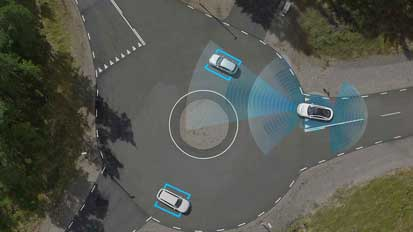
\includegraphics[height=2.25cm]{fig/ALV_Radar-Detection}
			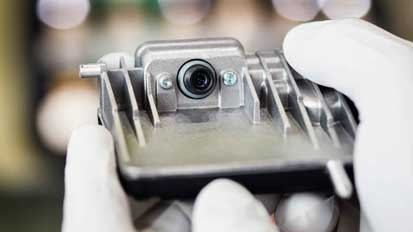
\includegraphics[height=2.25cm]{fig/ALV_Mono-Vision-Sensor}
			\caption{Copyright Autoliv}
		\end{figure}
	\end{columns}
\end{frame}

\begin{frame}{Mono compared to Stereo Vision}
	\begin{columns}
		\column{0.5\textwidth}
		Mono vision
		\begin{itemize}
			\item[$+$] Object detection
			\item[$+$] Less expansive
			\item[$-$] Lacking depth information
			\item[$-$] Increased algorithm complexity
		\end{itemize}
		\column{0.4\textwidth}
		\begin{center}
			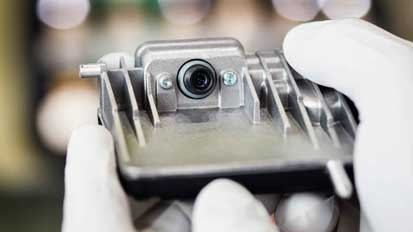
\includegraphics[width=3cm]{fig/ALV_Mono-Vision-Sensor}
		\end{center}
	\end{columns}
	\vspace{1em}
	\begin{columns}
		\column{0.5\textwidth}
		Stereo vision
		\begin{itemize}
			\item[$+$] Object detection
			\item[$+$] Depth information
			\item[$-$] More expensive
		\end{itemize}
		\column{0.4\textwidth}
		\begin{center}
			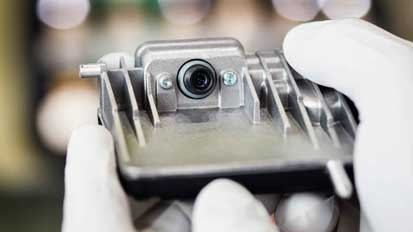
\includegraphics[width=2.25cm]{fig/ALV_Mono-Vision-Sensor}
			\hfill
			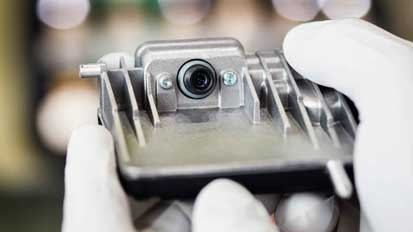
\includegraphics[width=2.25cm]{fig/ALV_Mono-Vision-Sensor}
		\end{center}
	\end{columns}
\end{frame}

\begin{frame}{Objective of the Master's Thesis}
	Since depth information is available in the stereo camera, orientation and angular rate are easy to estimate.
	How can we do that in a mono camera system?
	\pause
	\begin{block}{Objective}
		\begin{itemize}
			\item Can the heading (orientation and angular rate) of a vehicle be estimated using a mono camera system?
			\item Which kind of algorithms and models are suitable for solving the problem?
			\item How does a mono camera system performs compared with a stereo camera system?
		\end{itemize}
	\end{block}
\end{frame}

\begin{frame}{Limitations}
	\begin{itemize}
		\item The algorithm is not required to work in real-time
		\item Perfect knowledge about the ego car's ego motion
		\item Evaluated only on cars
		\item The size of the cars are known
	\end{itemize}
\end{frame}

% ------------------------------
\section{Theory and Methodology}
% ------------------------------

% ---------------
\section{Results}
% ---------------

% -------------------
\section{Conclusions}
% -------------------

\end{document}